\section{Imaging}
\label{sec:imaging}

% http://en.wikipedia.org/wiki/Free_induction_decay
% In Fourier Transform NMR, a free induction decay (FID) is the
% observable NMR signal generated by non-equilibrium nuclear spin
% magnetisation precessing about the magnetic field (conventionally
% along z). 

The observable signal used for imaging is a free induction decay, FID,
generated by non-equilibrium nuclear spin magnetization precessing
about the magnetic field

% B1 magnetic field

%% To distinguish slices in the body, a gradient field, $B_{G_s}$, is applied
%% along the z-axis. The gradient field varies along the z-axis, with
%% only a 0 Tesla effect in the slice that should be excited. Since the
%% frequency of the photons that can excite a spin is linearly
%% proportional to the strength of the magnetic field on that spin, it
%% follows that the photons of frequency $\omega_0 = \gamma B_0$ will
%% only affect spin packets unaffected by the gradient $B_{G_s}$. Applying
%% $B_{G_s}$ for the duration of the RF pulse ensures that only spin packets
%% in the slice is excited and will produce a signal during the signal
%% acquisition phase.



By Faraday's law of induction the signal generated by a single spin
packet is\footnote{\cite{feeman}}

\begin{displaymath}
  M^*(t, \mathbf{p}) = M_x(t, \mathbf{p}) + i \cdot M_y(t, \mathbf{p})
\end{displaymath}

The complete signal from the excited slice is then

\begin{displaymath}
    M^*(t) = \sum^{(X, Y)}_{(x',y')} (M_x(t, \mathbf{p_{(x',y')}}) + i \cdot M_y(t, \mathbf{p_{(x',y')}}))
\end{displaymath}

which is sampled in intervals of $t$ for the duration $\tau$.


The number of samples taken during each excitation is directly
proportional to the image resolution along the x-axis. The resolution
along the y-axis is given by how many times a slice is excited and
sampled.


\subsection{K-space}

The signal acquired is stored in K-space. Each specific excited slice
in the patient corrosponds to a two dimensional K-space image with
complex entries. A row in the image along the x-axis, the frequency
encoding direction, hold signals sampled over time $\tau$ at intervals
$t$ after one application of the RF pulse. All the lines along the
y-axis, the phase encoding direction, represent samples with different
phase encodings. An example of a K-space image can be seen in
\reffig{fig:kSpace}, where two net mangnetizations have produced a
signal.

With the information in K-space it is possible to restore the original
hydrogen intensities from the sampled FID signal. Fourier transforming
the image in \reffig{fig:kSpace} in its frequency encoding direction,
yields the frequency domain information seen in
\reffig{fig:frequencyDomain}. Fourier transforming this in the phase
encoding direction will give us the hydrogen intensities of the spin
packets, as can be seen in \reffig{fig:phaseDomain}. Here we can also
see why the phase encoding gradient varies for each excitation, as
that gives the oscilation along the phase encoding direction.


% Perform 2D fourier transform of the data in k-space, cuda does this
% with Sangilds wrapper

\begin{figure}
  \centering
  \subfigure[K-space]{
    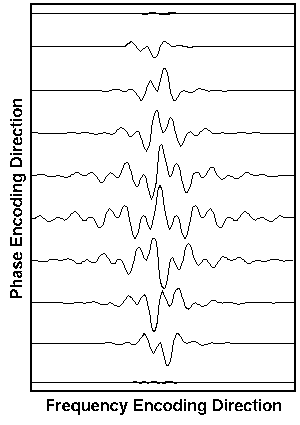
\includegraphics[width=4.5cm]{kSpace}
    \label{fig:kSpace}
  }
  \subfigure[Frequency domain information extracted by performing a
    Fourier transform along the x-axis.]{
    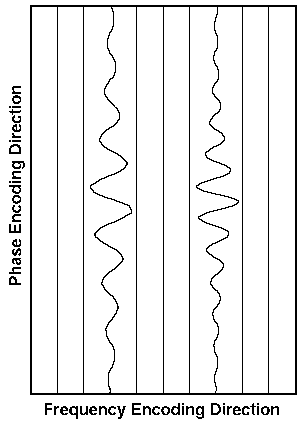
\includegraphics[width=4.5cm]{frequencyDomain}
    \label{fig:frequencyDomain}
  }
  \subfigure[Frequency and phase domain information extracted by performing a
    2D Fourier transform along the x- and y-axis.]{
    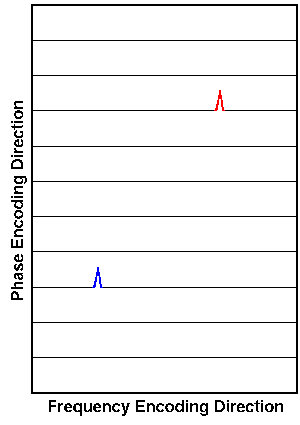
\includegraphics[width=4.5cm]{phaseDomain}
    \label{fig:phaseDomain}
  }
  \caption{The effect from fourier transforming a K-space image.}
  \label{fig:kSpaceTransformations}
\end{figure}

The one dimensional fourier transform is given by 

\begin{displaymath}
  \begin{array}{rl}
    f(\omega) &= \int^\infty_{-\infty}f(t)e^{-i \omega t} dt \\
    &= \int^\infty_{-\infty}f(t)(\cos(\omega t) - i \sin(\omega t)) dt \\
    &\approx \sum^\infty_{-\infty}f(t)(\cos(\omega t) - i \sin(\omega t))
  \end{array}
\end{displaymath}

% The signal strength is the length of the complex number from the
% fourier transform, not just the real component.

Since the fourier transform is both applied to and returns complex
numbers, the hydrogen intensity produced by a two dimensional
transform is also a complex number, $h'$. Converting this to the
final intensity, $h$, is done by taking the modulus of the complex
intensity.

\begin{displaymath}
  h = \|h'\| = \|h'_{real} + i h'_{imaginary}\| = \sqrt{h_{real}^{'2} + i h_{imaginary}^{'2}}
\end{displaymath}


%%% Local Variables:
%%% mode: latex
%%% TeX-master: t
%%% TeX-PDF-mode: t
%%% End:
